\documentclass{beamer}
\mode<presentation>
\usetheme{CambridgeUS}
\usepackage[russian]{babel}
\usepackage[utf8]{inputenc}
\usepackage[T2A]{fontenc}
\usepackage{sansmathaccent}

\usepackage{verbatim}
\usepackage{alltt}

\pdfmapfile{+sansmathaccent.map}
\title[СУБД]{Структуры базы данных. Часть~1. }
\author{Наумов Д.А., доц. каф. ИТГД, доц. каф. КТ}
\date[15.02.2019] {Основы компьютерных наук (3 часть), 2019}

\begin{document}

%ТИТУЛЬНЫЙ СЛАЙД
\begin{frame}
  \titlepage
\end{frame}
  
%СОДЕРЖАНИЕ ЛЕКЦИИ
\begin{frame}
  \frametitle{Содержание лекции}
  \tableofcontents  
\end{frame}
  
%РАЗДЕЛ 1
\section{План дисциплины}
\begin{frame}
Разделы дисциплины 'Основы компьютерных наук', 3-ий семестр обучения:
\begin{itemize}
\item \textbf{Структуры базы данных}. (\textit{24 часа}) Общие понятия. Многоуровневый подход к реализации баз данных. Реляционная модель. Объектно-ориентированные базы данных. 
\item \textbf{Операционные системы}. (\textit{24 часа}) Однопроцессорные системы. Многопроцессорные системы. Классификация программного обеспечения. Функции операционных систем. История развития ОС.
\item \textbf{Основы технологии разработки программного обеспечения}. (\textit{16 часов}) Жизненный цикл ПО. Стадии жизненного цикла. Модульность. Методы проектирования. Нисходящие и восходящие методы разработки.
\end{itemize}
\end{frame} 
  
\section*{Литература}
\begin{frame}   
Рекомендуемая литература:
\begin{enumerate}
\item Карпова Т. С. Базы данных: модели, разработка, реализация. — СПб.: Питер,. 2002. — 304 с., ил.
\item Базы данных : учебник для прикладного бакалавриата / Б. Я. Советов, В. В. Цехановский, В. Д. Чертовской. — 2-е изд. — М. : Издательство Юрайт, 2015. — 463 с. — Серия : Бакалавр. Прикладной курс
\item Дейт К. Дж. Введение в системы баз данных, 8-е издание.: Пер. с англ. — М.: Издательский дом "Вильямс", 2005. — 1328 с.: ил.
\item Тарасов С. В. СУБД для программиста. Базы данных изнутри. — М.: СОЛОН-Пресс, 2015. — 320 с.: ил.
\item Программирование  баз  данных  SQL.  Типичные  ошибки  и  их устранение  /  Б.  Карвин.  —  М.:  Рид  Групп,  2012.  — 336с. 
\end{enumerate}
\end{frame}   

\section{Основные понятия и определения}
\begin{frame}
\begin{itemize}
\item База данных (БД) — структурированное поименованное хранилище информации.
\end{itemize}
Пример: файл CSV? файл с текстом лекции?
\begin{itemize}
\item Система управления базами данных (СУБД) — специализированное программное обеспечение, обеспечивающее доступ к базе данных как к совокупности её структурных единиц.
\end{itemize}
Пример: текстовый редактор для CSV-файла? LibreOffice Calc для CSV-файла?
\end{frame} 

\begin{frame}
\begin{block}{Пример базы данных}
\begin{center}
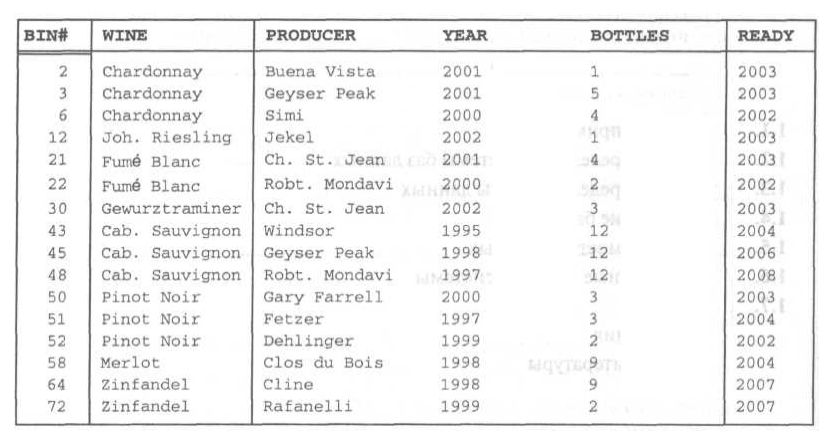
\includegraphics[scale=0.5]{images/example-01.png}
\end{center}
\end{block}
\end{frame} 

\begin{frame}
Базу данных можно рассматривать как подобие \textit{электронной картотеки}, т.е. хранилище или контейнер для некоторого набора файлов данных, занесенных в компьютер.

Пользователям СУБД предоставляется возможность выполнять (или передавать системе запросы на выполнение) множество различных операций над данными:
\begin{itemize}
\item добавлять пустые "файлы";
\item вставлять новые данные в существующие "файлы";
\item получать данные из существующих "файлов";
\item удалять данные из существующих "файлов";
\item изменять данные в существующих "файлов";
\item удалять существующие "файлов" из базы данных;
\end{itemize}
\end{frame}

\begin{frame}
\begin{block}{Пример выборки информации из базы данных}
\begin{center}
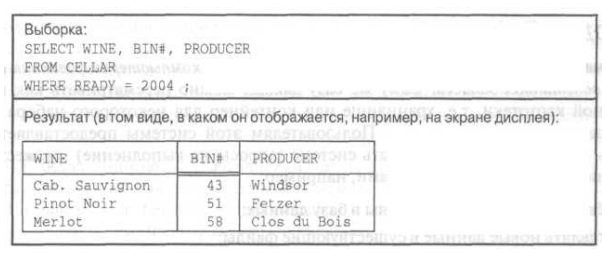
\includegraphics[scale=0.5]{images/example-02.png}
\end{center}
\end{block}
Язык SQL (\textit{Structured Query Language}, язык структурированных запросов)был первоначально разработан компанией IBM, а в настоящее время поддерживается большинством коммерческих СУБД, представленных на рынке, и является официальным стандартом языка для работы с реляционными базами данных.
\end{frame} 

\begin{frame}
\begin{block}{Примеры операций вставки, удаления и обновления}
\begin{center}
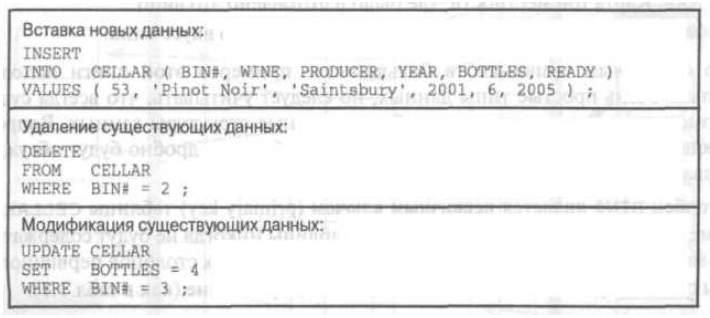
\includegraphics[scale=0.5]{images/example-03.png}
\end{center}
\end{block}
Используемые термины:
\begin{itemize}
\item файлы, записи.
\item таблицы, строки, столбцы.
\item отношения, кортежи и атрибуты.
\end{itemize}
\end{frame}

\begin{frame}
В примере предполагается, что в столбцах WINE и PRODUCER содержатся строковые данные, а во всех остальных столбцах — целочисленные данные. Но, как правило, столбцы могут содержать
данные произвольной сложности:
\begin{itemize}
\item LABEL. Фотография этикетки винной бутылки.
\item REVIEW. Текст отзыва о качестве вина, полученный из определенного винного
магазина.
\item MAP. Карта той местности, где было изготовлено это вино.
\item NOTES. Звукозапись, содержащая комментарии о вкусе вина.
\end{itemize}
Столбец BIN\# является \textbf{первичным ключом} (primary key) таблицы CELLAR (подразумевается, что любые две строки этой таблицы никогда не будут содержать одно и то же значение поля BIN\#)
\end{frame}

\begin{frame}
\begin{block}{Упрощенная схема СУБД}
\begin{center}
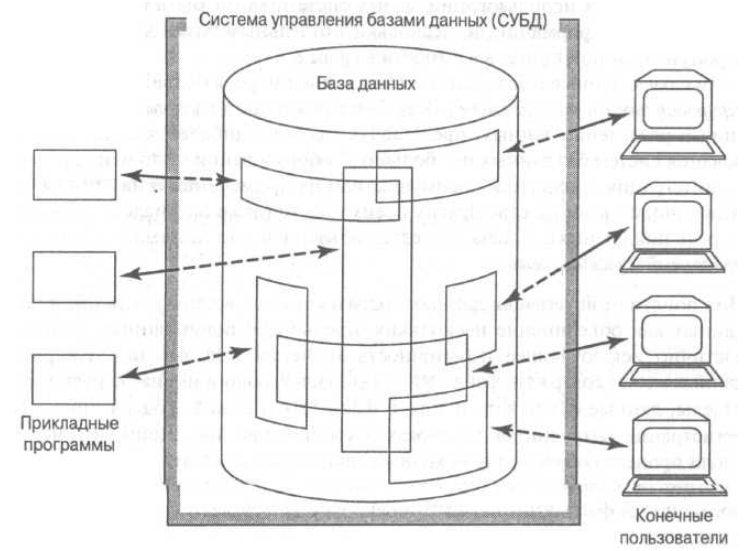
\includegraphics[scale=0.5]{images/shema-01.png}
\end{center}
\end{block}
\end{frame}

\begin{frame}
Четыре главных компонента СУБД:
\begin{itemize}
\item данные;
\item аппаратное обеспечение;
\item программное обеспечение;
\item пользователи.
\end{itemize}

Однопользовательская система (single-user system) — это система, в которой к базе данных может получить доступ одновременно только один пользователь. 

Многопользовательская система (multi-user system) — это такая система, в которой к базе данных могут получить доступ сразу несколько пользователей.

В общем случае данные в базе данных (по крайней мере, в больших системах) являются:
\begin{itemize}
\item интегрированными - подразумевается возможность представить базу
данных как объединение нескольких отдельных файлов данных, полностью или частично исключающее избыточность хранения информации.
\item разделяемыми - подразумевается возможность использования несколькими различными пользователями отдельных элементов, хранимых в базе данных.
\end{itemize}
\end{frame}

\begin{frame}
К аппаратному обеспечению системы относится:
\begin{itemize}
\item тома вторичной (внешней) памяти (обычно это магнитные диски), используемые
для хранения информации, а также соответствующие устройства ввода—вывода
(дисководы и т.п.), контроллеры устройств, каналы ввода—вывода и т.д.;
\item аппаратный процессор (или процессоры) вместе с оперативной (первичной) памятью, предназначенные для поддержки работы программного обеспечения системы
баз данных.
\end{itemize}
\end{frame}

\begin{frame}
\begin{itemize}
\item Между физической базой данных (т.е. данными, которые реально хранятся на компьютере) и пользователями системы располагается уровень программного обеспечения, который можно называть по-разному: диспетчер базы данных (database manager), сервер базы данных (database server) или, что более привычно, система управления базами данных, СУБД (DataBase Management System — DBMS).
\item Основная задача СУБД — дать пользователю базы данных возможность работать с ней, не вникая во все подробности работы на уровне аппаратного обеспечения. 
\item СУБД позволяет конечному пользователю рассматривать базу данных как объект более высокого уровня по сравнению с аппаратным обеспечением, а также предоставляет в его распоряжение набор операций, выражаемых в терминах языка высокого уровня.
\end{itemize}
\end{frame}

\begin{frame}
Пользователей можно разделить на три большие и отчасти перекрывающиеся группы:
\begin{itemize}
\item прикладные программисты, которые отвечают за написание при кладных программ, использующих базу данных.
\item конечные пользователи, которые работают с системой баз данных в интерактивном режиме. 
\item  администраторы базы данных.
\end{itemize}
\end{frame}

\begin{frame}
Исторически, в устройстве СУБД выделяли три уровня, предложенных ещё в 1975 году в отчёте ANSI/X3/SPARC:
\begin{itemize}
\item внешний уровень наиболее близок к приложениям и пользователям, он связан со специфичными для них способами представления данных.
\item логический уровень, также называемый концептуальным, для описаний данных, не зависящих от физической реализации; 
\item логический уровень, также называемый концептуальным, для описаний данных, не зависящих от физической реализации.
\end{itemize}
Внутренний уровень не всегда связан с файловой системой. Наиболее развитые современные СУБД представляют собой по сути специализированную операционную систему, способную управлять
физическими устройствами хранения, кешем данных, процессами и потоками, оперативной памятью, асинхронным запуском и внутренним планировщиком задач минуя собственно операционную систему
компьютера.
\end{frame}

\section{Типы приложений: транзакционная и аналитическая обработка}
\begin{frame}
\textbf{Транзакцией} в СУБД называется совокупность операций над данными, являющаяся неделимой (атомарной).

Отличительные особенности транзакционных приложений:
\begin{itemize}
\item Обработка идёт в режиме реального или приближенного к реальному времени. Время отклика системы при запросе оператора не превышает единиц секунд.
\item Запросы представляют собой интенсивный поток коротких операций по вставке, изменению и удалению небольшого числа записей в БД. Эти операции могут быть как одиночными транзакциями, так и объединяться в более крупные транзакции.
\end{itemize}
В реляционной СУБД любой оператор SQL является одиночной транзакцией по умолчанию.
OLTP (On-Line Transaction Processing) — собственно интерактивная транзакционная обработка.
ACID (Atomicity-Consistency-Isolation-Durability) — принципы неделимости, целостности,
изолированности и надёжности.
\end{frame}

\begin{frame}
аналитическая обработка данных имеет следующие отличительные признаки:
\begin{itemize}
\item Данные находятся \textbf{в режиме чтения}, за исключением моментов их обновления.
\item Выборки представляют собой \textbf{одиночные тяжёлые запросы}: поиски и расчёты по множеству произвольных критериев могут охватывать значительную часть данных в базе.
\item \textbf{Время отклика системы не регламентировано}, нередко пользователь имеет возможность прервать слишком долго.
\item Размеры базы данных, как правило, на порядок и больше превышают таковые для транзакционной.
\end{itemize}
Аббревиатурой для интерактивной аналитической обработки является OLAP (On-Line Analytical Processing). Соответственно, \textbf{интерактивное} приложение, работающее с СУБД в режиме OLAP, относится к аналитическим.
\end{frame}

\begin{frame}
\begin{block}{Пример диаграммы "Сущность-связь"}
\begin{center}
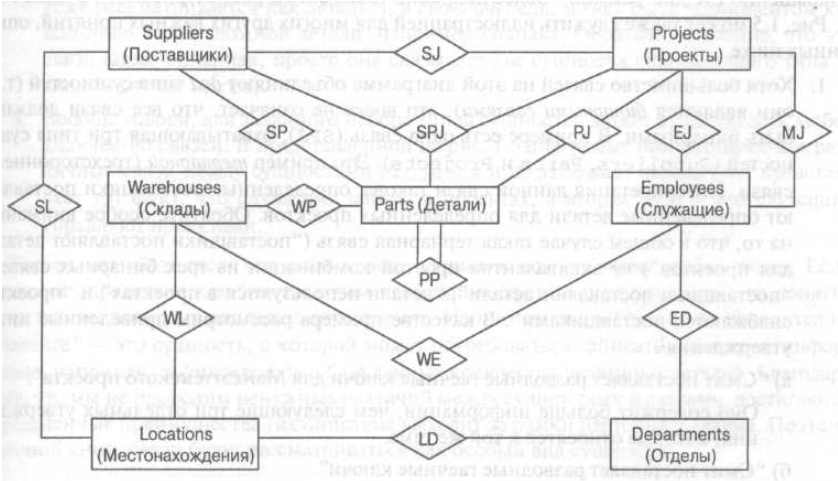
\includegraphics[scale=0.5]{images/shema-02.png}
\end{center}
\end{block}
\end{frame}

\section{Основные модели данных}

\begin{frame}
\begin{block}{Модель данных}
это абстрактное, самодостаточное, логическое определение объектов, операторов и прочих элементов, в совокупности составляющих абстрактную машину доступа к данным, с которой взаимодействует пользователь. Упомянутые объекты позволяют моделировать структуру данных, а операторы — поведение данных.
\end{block}
\begin{block}{Реализация (implementation) заданной модели данных}
это физическое воплощение на реальной машине компонентов абстрактной машины, которые в совокупности составляют эту модель.
\end{block}
Термин модель данных (иногда, некорректно) встречается в литературе другом толковании: модель данных представляет собой модель перманентных данных некоторого конкретного предприятия.
\end{frame}

\begin{frame}
\begin{block}{Классификация моделей данных [Карпова Т., Базы данных]}
\begin{center}
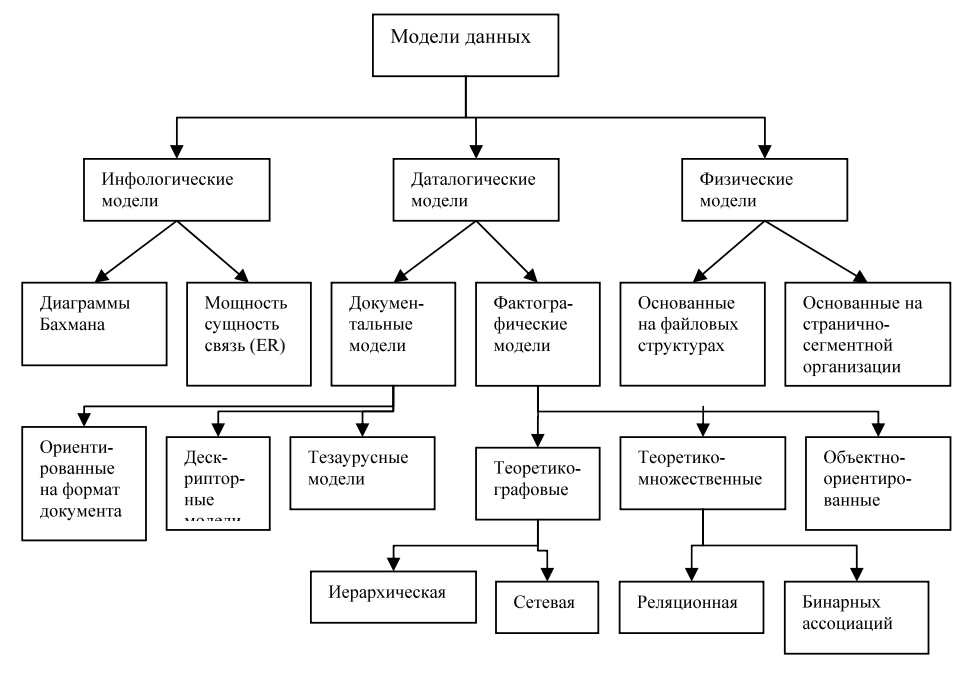
\includegraphics[scale=0.35]{images/shema-03.png}
\end{center}
\end{block}
\end{frame}

\begin{frame}
\begin{block}{Иерархическая модель}
- исторически, первая моделью данных, (т.е. способ их организации, структурирования, доступа и манипуляции данных).
\end{block}
IMS (Information Management System) фирмы IBM Разработанная в 1966 году до сих пор эксплуатируется на новейших мэйнфреймах серии Z, обеспечивая высокую производительность обработки порядка сотни тысяч транзакций в секунду.

Современной массово доступной каждому программисту реализацией иерархической модели данных является XML, точнее, разнообразные «движки» и API для манипуляции со структурами, созданными на основе этой технологии с обязательным применением схем определения данных.
\end{frame}

\begin{frame}
\begin{block}{Пример XML-документа}
\begin{center}
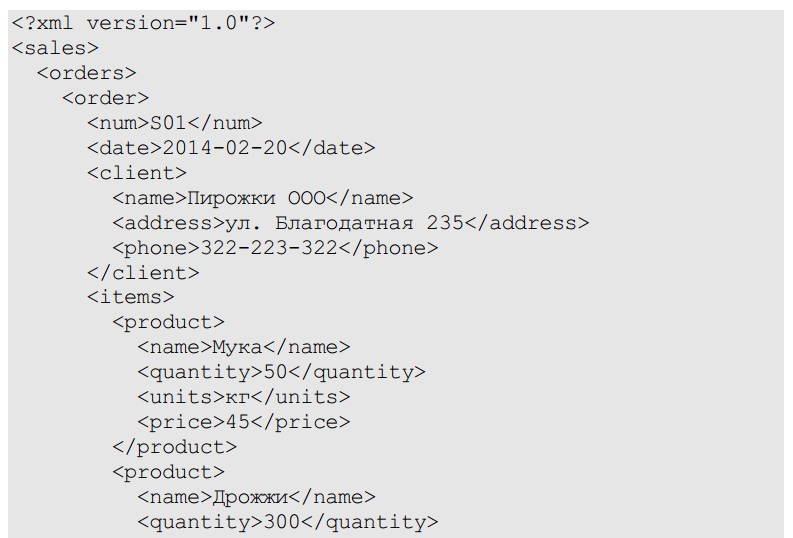
\includegraphics[scale=0.5]{images/example-04.png}
\end{center}
\end{block}
\end{frame}

\begin{frame}
\begin{block}{Пример запроса к данным XML-документа}
\begin{center}
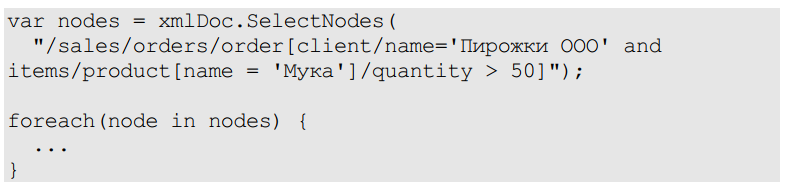
\includegraphics[scale=0.5]{images/example-05.png}
\end{center}
\end{block}

Если при использовании входного языка и/или API наиболее низкого уровня из доступных программисту для доступа к данным (значениям узлов, переменных, полей и т. д.) \textbf{требуется указывать некоторый путь}, то лежащая в основе СУБД модель базируется на \textbf{иерархиях}.
\end{frame}

\begin{frame}
\begin{block}{Преимущества иерархической модели}
\begin{itemize}
\item отнести относительную простоту восприятия логической структуры базы данных человеком.
\item высокое быстродействие при транзакционной обработке, когда номенклатура типов запросов фиксирована.
\end{itemize}
\end{block}
\begin{block}{Недостатки иерархической модели}
\begin{itemize}
\item медленный доступ к данным нижних уровней иерархии;
\item чёткая ориентация структур на определённые типы запросов, что исключает универсальность использования одной и той же БД разными типами приложений;
\item модель графов ограничена деревьями, что сужает область её применения.
\end{itemize}
\end{block}
\end{frame}

\begin{frame}
\begin{block}{Сетевая модель}
Сетевую модель можно представить в виде графа с узлами в виде записей, и рёбрами, отображающими наборы.
\end{block}
До наших дней дожило только небольшое число СУБД, реализующих сетевую модель, например американская Raima (бывшая dbVista) и отечественная КроносПро.
\end{frame}

\begin{frame}
\begin{block}{Запись}
соответствует аналогичному понятию структурного типа в традиционных языках программирования: record в Паскаль-подобных или struct в наследниках Си.
\end{block}
\begin{block}{Набор данных}
служит для связывания двух типов записей отношением «один-ко-многим».
\end{block}
\begin{block}{Организация связей в сетевой модели}
\begin{center}
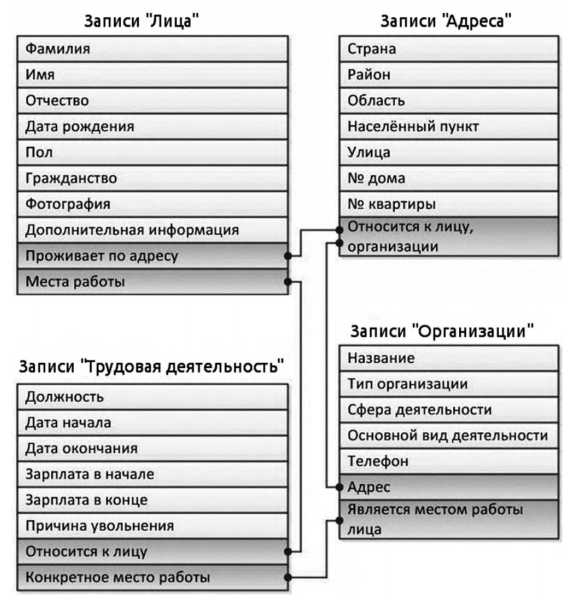
\includegraphics[scale=0.25]{images/shema-04.png}
\end{center}
\end{block}
\end{frame}

\begin{frame}
\begin{block}{Преимущества сетевой модели}
\begin{itemize}
\item стандартизация. Стандарт CODASYL определяет базовые понятия модели и формальный язык описания.
\item быстродействие сетевых БД данных сравнимо с таковым для иерархических БД.
\item Полное использование теоретико-графовых моделей предоставляет высокий уровень абстракции описания предметных областей, не ограниченных иерархиями.
\item гибкость доступа к данным через любую последовательность связанных записей, а не через их иерархию.
\end{itemize}
\end{block}
\begin{block}{Недостатки сетевой модели}
\begin{itemize}
\item жёсткость задаваемых структур и сложность реструктуризации схем БД.
\item сложная структура управления памятью в транзакционных приложениях с частыми изменениями связей.
\end{itemize}
\end{block}
\end{frame}

\end{document}
